% http://tex.stackexchange.com/questions/11866/compile-a-latex-document-into-a-png-image-thats-as-short-as-possible#11880
%http://tex.stackexchange.com/questions/152247/best-practice-to-include-standalone-precompiled-graphics
\documentclass[border=1pt]{standalone}
\usepackage{tikz}

\begin{document}

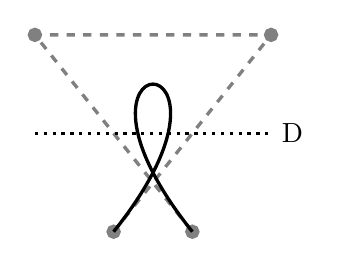
\begin{tikzpicture}[very thick]
	\newcommand {\hy} {2.5}
	\coordinate (s1) at (1,0); \coordinate (s2) at (3,\hy);
	\coordinate (s3) at (0,\hy); \coordinate (s4) at (2,0);
	\draw[dashed, gray] (s1) -- (s2) -- (s3) -- (s4);
	\foreach \x in {s1,s2,s3,s4}
	{
		\draw[fill=white, gray] (\x) circle [radius=2pt];
	}
	\draw (s1) .. controls (s2) and (s3) .. (s4);
	\draw[dotted] (0, 0.5*\hy) -- (3,0.5*\hy) node[right] {D};
\end{tikzpicture}

\end{document}
